\documentclass[11pt]{article}

\author{Groep 6:\\
		Niels Desair\\
		Bram Kelchtermans\\
		Dylan Toirkens}
		
\title{\textbf{Studie van meetbare objectieven en ontwerpprincipes van Shneidermann}}

\date{19/10/2016}

\usepackage{graphicx}
\usepackage{parskip}
\usepackage{float}

\begin{document}
	\begin{titlepage}
		
		\newcommand{\HRule}{\rule{\linewidth}{0.5mm}} % Defines a new command for the horizontal lines, change thickness here
		
		\begin{center} % Center everything on the page
			
			\textsc{\LARGE Universiteit Hasselt}\\[1.5cm] % Nme of your university/college
			\textsc{\Large Humane en sociale aspecten van de informatica}\\[0.5cm] % Major heading such as course name
			
			\HRule \\[0.4cm]
			{ \huge \bfseries Studie van meetbare objectieven en ontwerpprincipes van Shneidermann}\\[0.4cm]
			\HRule \\[1.5cm]
			
			\begin{minipage}{0.4\textwidth}
				\begin{flushleft} \large
					\emph{Groep 6:}\\
					Niels \textsc{Desair} \newline
					Bram \textsc{Kelchtermans} \newline
					Dylan \textsc{Toirkens}
				\end{flushleft}
			\end{minipage}
			~
			\begin{minipage}{0.4\textwidth}
				\begin{flushright} \large
					\emph{Datum:}\\
					19 Oktober 2016
					\emph{Academiejaar: } \\
					2016-2017
				\end{flushright}
			\end{minipage}\\[4cm]
			\vspace{40 mm}
			\includegraphics[width=3.0cm]{uhasselt-logo}\\[2.0cm]  
		\end{center}
	\end{titlepage}

\section{Inleiding}
Voor het vak Humane en Sociale Aspecten van de Informatica is ons gevraagd om twee applicaties te vergelijken. Dit op het vlak van de ontwerpprincipes van Norman en op het vlak van metaforen. Deze paper zal bestaan uit drie individuele delen waarna we afsluiten met een gezamelijke conclusie. We hebben besloten om de communicatieapplicaties Skype en Google Hangouts te bespreken. We gebruiken de Google Hangouts extensie, dus niet de website.
\newpage

\section{Bespreking Niels}
Individuele bespreking (twee tot drie bladzijden, 800 à 1200 woorden)
\subsection{Ontwerpprincipes van Norman}
\subsubsection{Visibility}
\subsubsection{Feedback}
\subsubsection{Affordance}
\subsubsection{Mapping}
\subsubsection{Constraints}
\subsection{Metaforen}
\newpage

\section{Bespreking Bram}
\subsection{Ontwerpprincipes van Norman}
\subsubsection{Visibility}
Visibility wil zeggen dat alle mogelijke acties en opties meteen zichtbaar moeten zijn voor de gebruiker. Persoonlijk vind ik dat Google Hangouts op dit vlak verder staat dan Skype. Op Figuur \ref{fig:BeginHangouts} is het beginscherm van Hangouts te zien, meteen zijn ook alle functionaliteiten zichtbaar. Zo kan je een contactpersoon bellen, zoeken of toevoegen. Ook kan je zien welke gesprekken je de voorbije tijd gevoerd hebt en met wie. Een nadeel aan Skype is te zien op Figuur \ref{fig:BeginSkype}, zelf vind ik het zeer onduidelijk hoe men een contactpersoon moet zoeken of toevoegen. Wanneer men beter kijkt ziet men onder de eigen profielfoto een zoekvakje. In eerste instantie zou men denken dat dit enkel is om te zoeken, echter is dit ook bedoeld om contactpersonen toe te voegen. Persoonlijk vind ik dit zeker niet duidelijk voor een gebruiker die Skype niet kent. Wat dan wel in het voordeel van Skype speelt is het feit dat men kan kiezen tussen "contactpersonen" en "recent", dit terwijl bij Hangouts men vastzit aan "recent". Het is dus in Hangouts moeilijker om een overzichtelijke lijst van contacten te verkrijgen. Hangouts maakt dit dan wel goed door duidelijk een knop te voorzien om een nieuw gesprek te starten met (eventueel meerdere) contactpersonen.
\newline
De basisfuncties zoals bellen, chatten... zijn wel meteen en duidelijk zichtbaar in beide applicaties. De gebruiker selecteert of zoekt de gewenste contactpersoon en belt deze op met de daarvoor bestemde icoontjes. Deze icoontjes worden verder besproken in het deel "Affordance".
\begin{figure}
	\centering
	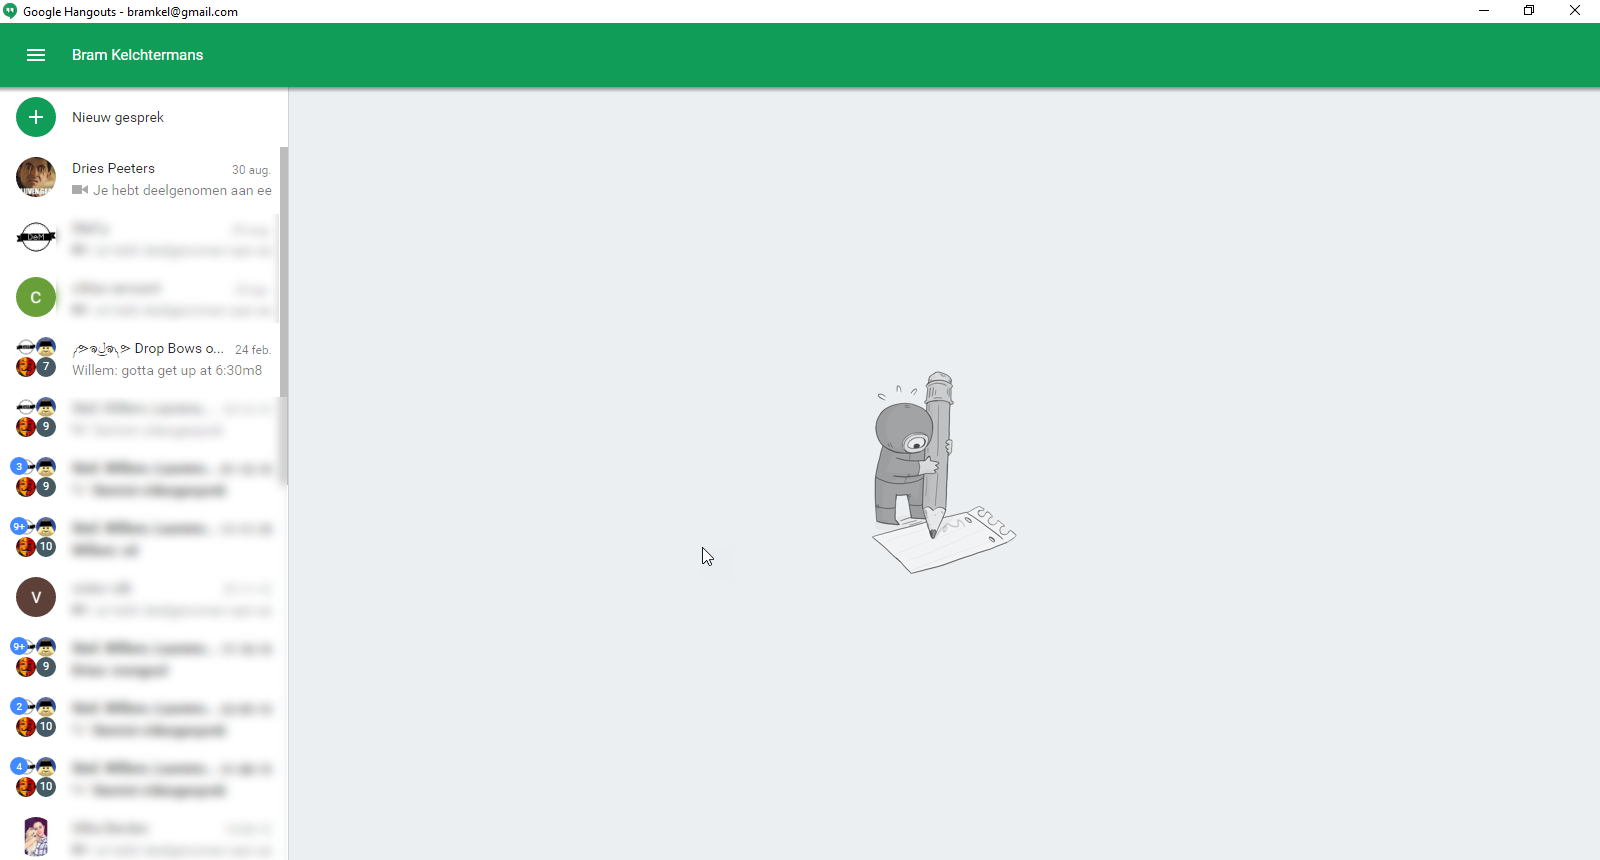
\includegraphics[width=1\textwidth]{Bram_ScreenshotGH1.png}
	\caption{Beginscherm van Hangouts}
	\label{fig:BeginHangouts}
\end{figure}
\begin{figure}
	\centering
	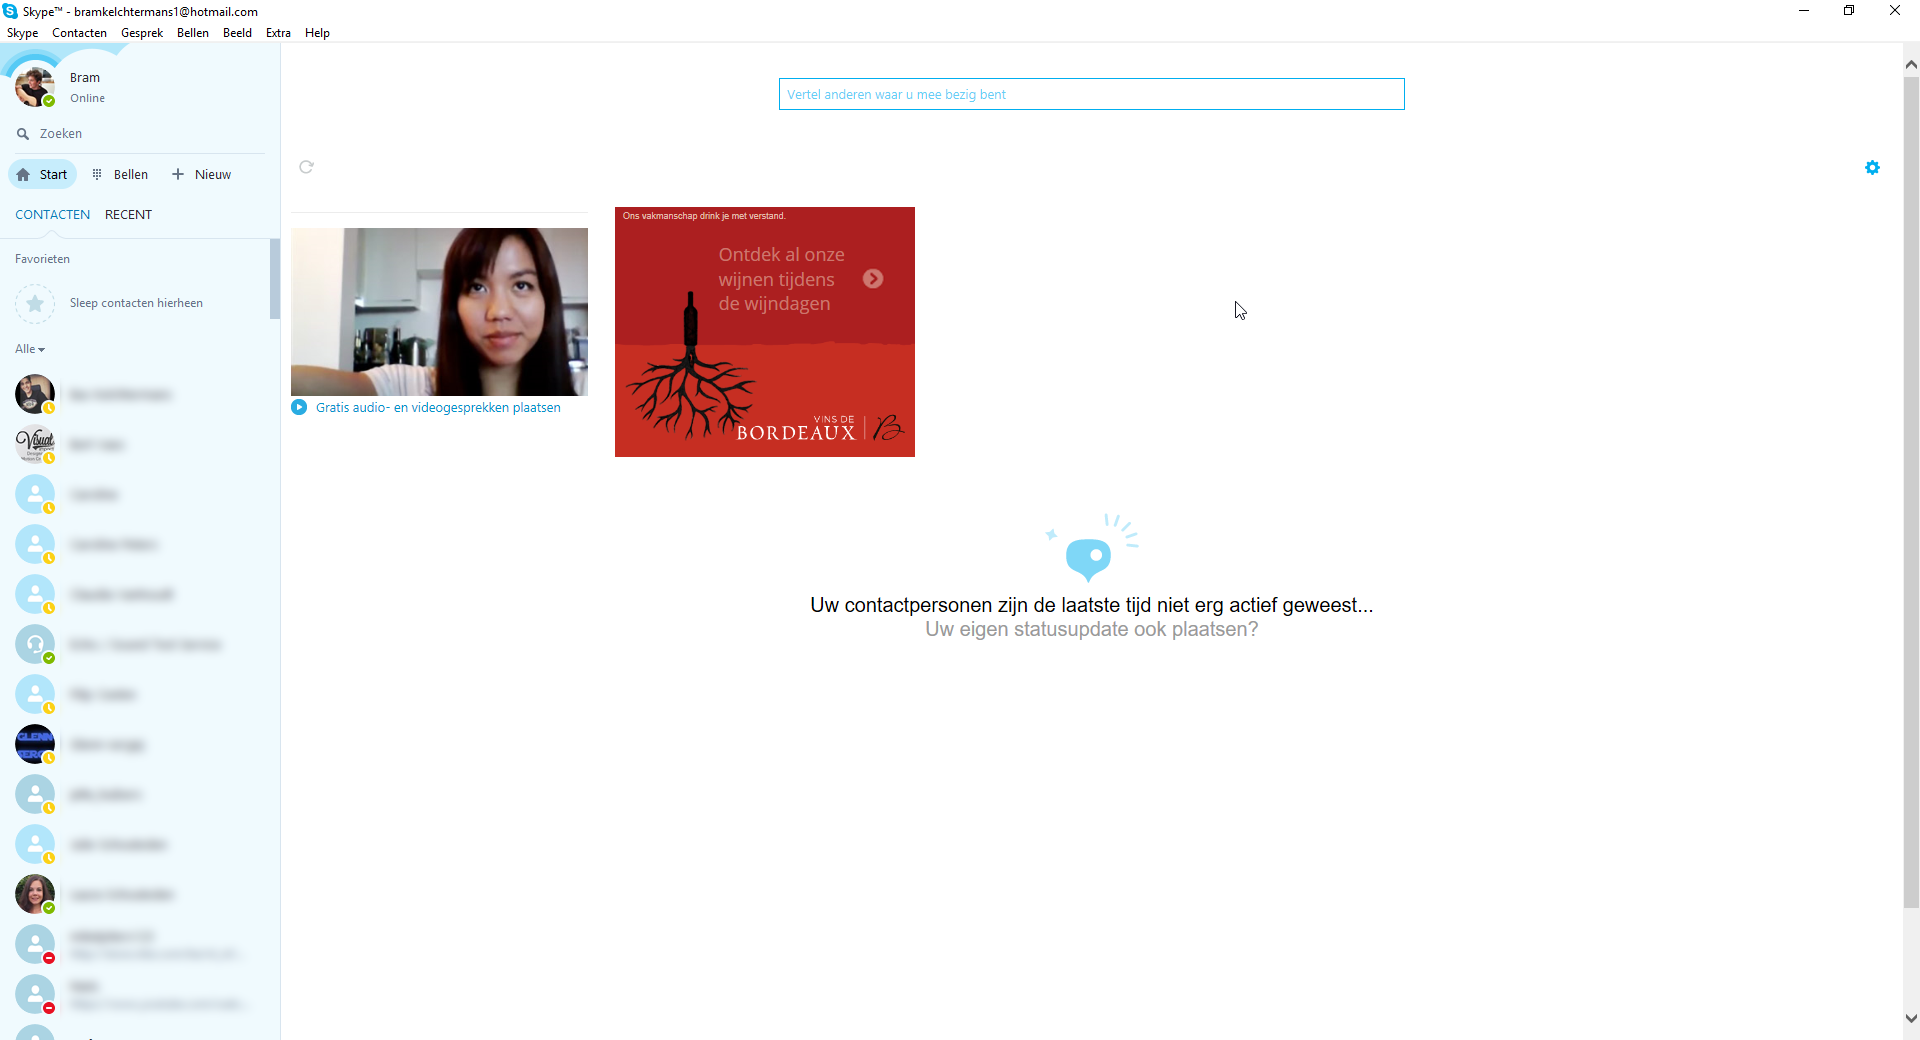
\includegraphics[width=1\textwidth]{Bram_ScreenshotSkype1.png}
	\caption{Beginscherm van Skype}
	\label{fig:BeginSkype}
\end{figure}
\subsubsection{Feedback}
Bij beide applicaties wordt er goed gebruik gemaakt van feedback. Dit vooral in de vorm van auditieve en tekstgebaseerde feedback. Zo wordt er telkens wanneer de gebruiker iemand belt een beltoon gespeeld, dit zodat de gebruiker weet dat de contactpersoon het verzoek om te bellen aan het ontvangen is. De ontvanger van de oproep hoort dan weer een beltoon op zijn of haar computer die aangeeft dat er iemand belt. Wanneer de contactpersoon echter niet bereikbaar is, krijgt de gebruiker duidelijk te horen dat de oproep niet beantwoord werd. Dit met een geluidstoon die duidelijk het einde van het gesprek aangeeft, ook krijgt de gebruiker een tekstgebaseerde feedback dat de contactpersoon niet bereikbaar is.
\newline
Een ander voorbeeld van feedback is te zien in figuur \ref{fig:VerzoekHangouts} voor Hangouts en in figuur \ref{fig:VerzoekSkype} voor Skype. In beide gevallen heeft de gebruiker een verzoek gestuurd om contactpersonen te worden met een persoon. Om te bevestigen dat de desbetreffende persoon een verzoek heeft ontvangen gebruiken beide applicaties een tekstboodschap als feedback. In beide applicaties wordt er in de chatsessie veel feedback gegeven. Zo ziet de gebruiker de volledige gespreksgeschiedenis met de geselecteerde contactpersoon. Dit gaat dan over gespreksduur, chatberichten...
\begin{figure}
	\centering
	
\includegraphics[width=0.7\textwidth]{Bram_ScreenshotGH2.png}
	\caption{Contactverzoek in Google Hangouts}
	\label{fig:VerzoekHangouts}
\end{figure}
\begin{figure}
	\centering
	
\includegraphics[width=0.7\textwidth]{Bram_ScreenshotSkype2.png}
	\caption{Contactverzoek in Skype}
	\label{fig:VerzoekSkype}
\end{figure}
\newline
Feedback is een zeer belangrijk aspect in deze context. Deze feedback is ook een soort metafoor aangezien de gebruiker dit kan mappen naar het brondomein: het telefoongesprek. In dit brondomein wordt er gebruik gemaakt van dezelfde soort auditieve feedback zoals de beltoon.
\subsubsection{Affordance}
Door het gebruik van metaforen en tekstgebaseerde GUI items is het snel duidelijk welke functie een bepaald element heeft. Zoals al eerder besproken heeft Skype een minpunt op dit vlak. Denk maar aan de zoekbalk van Skype, het is hier zeker niet duidelijk dat deze ook dient om nieuwe contacten te vinden. Bij Hangouts is dit echter wel duidelijk omdat er een grote knop met een "+" voorzien is, met de uitleg "Nieuw gesprek". Deze uitleg is belangrijker dan op het eerste zicht zou lijken, een nieuwe gebruiker zou bijvoorbeeld kunnen denken dat de knop enkel functie heeft om nieuwe contacten toe te voegen. 
\newline
Hangouts heeft echter ook een slechte affordance. Zoals te zien is in figuur \ref{fig:SoortHangouts} krijgt de gebruiker alleen de mogelijkheid om een videogesprek te starten. De gebruiker weet niet dat de camera tijdens het gesprek uitgeschakeld kan worden. Een nadeel is dus dat de gebruiker niet de mogelijkheid krijgt om een gesprek te starten zonder videobeelden.
\newline
 Verder is het wel duidelijk in beide applicaties hoe men een contactpersoon selecteert en deze dan kan contacteren. Ook is het duidelijk waar de gebruiker moet typen om een chatbericht achter te laten. 
 \subsubsection{Mapping}
 Bij het bellen via Skype of Hangouts kan je twee soorten gesprekken onderscheiden: spraakgesprekken of videogesprekken. Het is belangrijk dat de gebruiker duidelijk weet welk gesprek er gestart wordt. In figuur \ref{fig:SoortSkype} is de mapping duidelijk. De gebruiker krijgt de keuze welk soort gesprek er gestart zal worden. Deze mapping is ook van toepassing in Hangouts, hier wordt echter de nadruk gelegd op videogesprekken (zoals te zien is in figuur \ref{fig:SoortHangouts}).
 \begin{figure}
	\centering
	
\includegraphics[width=0.4\textwidth]{Bram_ScreenshotSkype3.png}
	\caption{Soorten gesprekken in Skype}
	\label{fig:SoortSkype}
\end{figure}
\begin{figure}
	\centering
	
\includegraphics[width=0.4\textwidth]{Bram_ScreenshotGH3.png}
	\caption{Soorten gesprekken in Hangouts}
	\label{fig:SoortHangouts}
\end{figure}
 \subsubsection{Constraints}
Beide applicaties hebben verschillende constraints. In Hangouts kan een gebruiker bijvoorbeeld niemand bellen die hem of haar niet geaccepteerd heeft als contactpersoon. Zo probeert Google te vermeiden dat er ongewenste gesprekken binnenkomen bij de gebruikers. Ook bij Skype is de mogelijkheid om een videogesprek te voeren met iemand die niet in de contactenlijst staat buiten werking gesteld. Het is echter wel nog mogelijk om een spraakgesprek te voeren met deze persoon. Persoonlijk vind ik dat Skype dit beter oplost, het kan zich namelijk voordoen dat je een persoon wilt contacteren die niet in je contactenlijst staat. Aangezien Skype deze mogelijkheid biedt in de vorm van een spraakgesprek is zeker een pluspunt.
\subsection{Metaforen}
Er zijn in beide applicaties duidelijke metaforen. Zo is het brondomein wel zeer duidelijk: het telefoongesprek. De icoontjes (zoals te zien in figuur \ref{fig:SoortSkype} en figuur \ref{fig:SoortHangouts}) maken duidelijk gebruik van de kennis van de gebruiker. Ook de geluiden zijn bekend voor de gebruiker, denk maar aan de wachttonen, beltonen... 
\newline
Als men als brondomein de mobiele telefoon neemt zijn er nog meer metaforen. Zo kan men tekst berichten versturen, zoals een SMS. Het versturen van een MMS is ook verwerkt in beide applicaties, de gebruiker kan namelijk foto's en video's versturen. 
\newline
Beide programma's hebben echter ook mismatches. Deze zijn echter bewust, denk zo aan de groepsgesprekken of de mogelijkheid om bestanden door te sturen. Deze functionaliteiten zorgen voor meer gebruiksgemak. 
\newline
Een recent toegevoegde functie aan beide applicaties is het achterlaten van een voicemail. Ook hier is een mismatch aanwezig aangezien de gebruiker ook een videobericht kan achterlaten voor de contactpersoon. Het spreekt voor zich dat dit niet het geval is bij een 'ouderwets' telefoongesprek.
\newpage

\section{Bespreking Dylan}
Individuele bespreking (twee tot drie bladzijden, 800 à 1200 woorden)
\subsection{Ontwerpprincipes van Norman}
\subsubsection{Visibility}
\subsubsection{Feedback}
\subsubsection{Affordance}
\subsubsection{Mapping}
\subsubsection{Constraints}
\subsection{Metaforen}
\newpage


\section{Conclusie}

\newpage
\end{document}